\documentclass[12pt]{article}
\usepackage[T1]{fontenc}
\usepackage[utf8]{inputenc}
\usepackage{graphicx} % includegraphics and all images tools
\usepackage{float}
\usepackage[intlimits]{amsmath}
\usepackage{amssymb,amsfonts}
% \usepackage{txfonts} arial 
\usepackage{fancyhdr} % Extensive control of page headers and footers
\usepackage{fancyvrb}
\usepackage{subcaption}
\usepackage{chngcntr}
\usepackage{hyperref} % links and urls in document
\usepackage{indentfirst} % wcięcie pierwszego akapitu

%begin tick and X emojis
\usepackage{pifont}
\usepackage{xcolor}
\newcommand{\cmark}{\textcolor{green!80!black}{\ding{51}}}
\newcommand{\xmark}{\textcolor{red}{\ding{55}}}
%end

%kolor linków
\hypersetup{
  colorlinks   = true, %Colours links instead of ugly boxes
  urlcolor     = black, %Colour for external hyperlinks
  linkcolor    = black, %Colour of internal links
  citecolor   = black %Colour of citations
}

\restylefloat{table}
\renewcommand{\contentsname}{Spis treści}
\renewcommand{\abstractname}{}
\renewcommand{\listfigurename}{}
\renewcommand{\listtablename}{}
\let\svaddcontentsline\addcontentsline


\renewcommand{\figurename}{Rys.}
\renewcommand{\tablename}{Tab.}
\renewcommand{\baselinestretch}{1.5}
% \setlength{\textwidth}{14cm}
% \setlength{\textheight}{20cm}
\numberwithin{figure}{section}
\counterwithin{table}{section}

\begin{document}
%------------------------------------------------
% Title page
%------------------------------------------------
\begin{titlepage}
 \thispagestyle{empty}
 \begin{center}
  \vspace{3cm}
  \large
    PRACA DYPLOMOWA INŻYNIERSKA\\
  \vspace{5cm}

  \Huge
    Aplikacja dla korepetytorów z płatnościami PayPal w technologii .NET Core\\
  \large
  \vspace{2cm}
  Bartosz Jurczewski, album 210209\\
  \bigbreak
  Politechnika Łódzka\\
  Wydział Fizyki Technicznej, Informatyki i Matematyki Stosowanej\\
  Rok akademicki 2019/2020\\
  \bigbreak
   dr hab inż Aneta Poniszewska-Marańda \\
 \end{center}
\end{titlepage}

\clearpage
\pagenumbering{arabic}
\setcounter{page}{1}
\setcounter{secnumdepth}{3}

%------------------------------------------------
% Main contents
%------------------------------------------------
\tableofcontents
\pagebreak

%%%%%%%%%%%%%%%%%%%%%%%%%%%%%%%%%%%%%%%%%%%%%%%%%%%%%%%%%%%%
%% Skróty użyte w pracy
%%%%%%%%%%%%%%%%%%%%%%%%%%%%%%%%%%%%%%%%%%%%%%%%%%%%%%%%%%%%
% \section{Skróty użyte w pracy}
% WebAPI - (ang. Web Application Programming Interfaces) Interfejs webowy, dla uproszczenia autor przyjmuje skrót API jako tożsamy.
% RESTful API
% Frontend - 
% Backend - 
% HTML
% CSS
% JavaScript
% Bootstrap
% HTTP
% JSON

\pagebreak
%%%%%%%%%%%%%%%%%%%%%%%%%%%%%%%%%%%%%%%%%%%%%%%%%%%%%%%%%%%%
%% Wprowadzenie
%%%%%%%%%%%%%%%%%%%%%%%%%%%%%%%%%%%%%%%%%%%%%%%%%%%%%%%%%%%%
\section{Wprowadzenie}
\textit{Otacza nas rewolucja cyfrowa. Każdy aspekt naszego życia przenosi się do internetu. Jednym z nich jest rynek usług - korepetycji. Aplikacja internetowa "Find-A-Tutor" jest odpowiedzią na tą rewolucję; pozwala na łatwe zarządzanie korepetycjami - dla ucznia i nauczyciela.}
% Wraz z początkiem lat 70 ubiegłego wieku świat ekonomi nie był już tylko kierowany przez prawa rynku ale także przez otaczający go i postępujący świat cyfryzacji, który z dnia na dzień zmieniał i na nowo definiował działania jego sektorów. 
% % Od samego początku cywilizacji Zachodniej, to niewątpliwie ekonomia jej towarzyszyła. 

% Nauką która zawsze towarzyszyła rozwojowi cywilizacji Zachodniej była ekonomia. To właśnie produkcja, konsumpcja czy dystrybucja dóbr napędzała 

% Świat ekonomii wraz z początkiem lat 70 ubiegłego wieku zaczął przechodzić transformacje.

% Wraz z początkiem lat 70 ubiegłego wieku świat ekonomi nie był już tylko kierowany przez prawa rynku
%%%%%%%%%%%%%%%%%%%%%%%%%%%%%%%%%%%%%%%%%%%%%%%%%%%%%%%%%%%%
%% Problematyka
%%%%%%%%%%%%%%%%%%%%%%%%%%%%%%%%%%%%%%%%%%%%%%%%%%%%%%%%%%%%
\subsection{Problematyka} \label{sec:problematyka}
Niewątpliwie czynnikiem który kształtował ekonomie, rynek czy cywilizacje zachodnią jako ogół była zawsze technologia. To ona bezpowrotnie zmieniła oblicze życia w latach 1780–1840 podczas rewolucji przemysłowej i to właśnie ona na nowo definiuje działania naszego świata podczas rewolucji cyfrowej. Początek tej rewolucji datowany jest na lata 70 XX wieku, ale jej koniec nie został jeszcze wyznaczony, ponieważ przyjmuje się, że trwa ona do dziś.

W roku 2019 prawie 60\% populacji świata miała dostęp do komputera \cite{internet-users}, a w samym 2019 zostało ich sprzedane prawie 230 tysięcy jednostek\cite{computers}. Obie te liczby przez ostatnie dekady miały tendencję wzrostową, co tylko jeszcze bardziej umacnia obecność technologi w naszym życiu. Niebywałą trudność może sprawić nam znalezienie takiej dziedziny życia która jeszcze nie została zmodyfikowana przedrostkiem "e" jako jednoznaczny sygnał cyfryzacji.

Pojęcie otaczającego nas wolnego rynku obejmuje również konkurencje. W warunkach idealnych, jest to model "konkurencji doskonałej", w którym to każdy z dostawców, swoją jakością produktu może rywalizować o pieniądze konsumenta. W dzisiejszych czasach konsument którego np. interesuje wybranie i zakup książki będzie miał do wyboru ponad 10 portali, takich jak \url{www.taniaksiazka.pl}, \url{swiatksiazki.pl}, \url{bonito.pl} czy \url{aros.pl}. Każdy z tych portali oferuje ponad 400 tysięcy pozycji jak i wiele udogodnień np. bezpłatny odbiór w jednej z 125 księgarni w Polsce \cite{ranking}. 

Przyglądając się innym branżom stosującym e-commerce (ang. handel elektroniczny) takim jak: AGD/RTV, artykuły medyczne, zoologiczne, dom i wnętrze, mililitra, motoryzacja, odzież i obuwie, sport, telefony, zdrowie i uroda, zegarki i biżuteria czy nawet żywność widzimy bogatość tych rozwiązań wraz z setkami udogodnień dla potencjalnego klienta. 

Obok rynku produktów znajduje się rynek usług. Najczęściej reprezentowany przez serwis aukcyjny lub ogłoszeniowy w którym to dany specjalista może zaoferować swój czas i umiejętności za określoną kwotę. Popularnymi i największymi portalami używanymi do tego są między innymi \url{olx.pl} lub \url{allegro.pl}.
Ze względu na specyfikę usługi, która nie jest namacalna tak jak produkt, przedstawienie jej w sposób dokładny może wiązać się z pewnymi trudnościami. Np. brak zdjęcia, brak możliwości zmierzenia jej jak produktu czy też po po prostu mniejsza ilość sposobów na opisanie jej. Sprawia to, że są one najczęściej dostępne jako dodatkowo opcja do serwisu handlowego. 

Specyficzną niszą są korepetycje. Oferowane nie tylko przez nauczycieli akademickich lub innych szkół, ale także studentów lub po prostu znawców danej dziedziny. Tradycyjnym sposobem znalezienia korepetytora było szukanie go przez polecenie lub znalezienie papierowego ogłoszenia. Kształt jak i długość lekcji były najczęściej dostosowywane dopiero przy spotkaniu z daną osobą.

Ostatnim analogowym aspektem korepetycji są oczywiście płatności - dokonywane gotówką. Płatność taka zajmuje zawsze więcej czasu, wiąże się często z wydawaniem reszty i jest nienamierzalna (zależnie od sytuacji jest to zaleta lub wada). Od strony płacącego wiążę się to z brakiem jakiekolwiek historii płatności, a od strony odbiorcy płatności związane jest z jakimkolwiek brakiem historii wpływów który np. pozbawia go możliwości analizowania jego działalności od strony finansowej. 

W tradycyjnym modelu korepetycji to nauczyciel ogłasza się jako osobo świadcząca te usługi. Brakuje jednak rozwiązań, a w szczególności w świecie cyfrowym, które pozwoliłby ogłaszać się uczniom jako poszukującym korepetycji. Takie rozwiązanie niewątpliwie powinno łączyć zalety serwisów ogłoszeniowych, odwrócony model ogłaszania się (jako ucznia która tych korepetycji poszukuje) i popularnych płatności on-line. Całość oczywiście powinna być spięta w prosty i intuicyjny interfejs który swoim minimalizmem nie przytłoczy użytkownika. Co często ma miejsce w serwisach powstałych kilka lat temu i zbyt bogatych w treść.
%%%%%%%%%%%%%%%%%%%%%%%%%%%%%%%%%%%%%%%%%%%%%%%%%%%%%%%%%%%%
%% Cel i założenia projektu
%%%%%%%%%%%%%%%%%%%%%%%%%%%%%%%%%%%%%%%%%%%%%%%%%%%%%%%%%%%%
\subsection{Cel i założenia projektu}
Bezpośrednim celem pracy jest dostarczenie aplikacji webowej która w łatwy sposób pozwoli na zarządzanie korepetycjami ze strony ucznia jak i nauczyciela. Aplikacja pozwoli nie tylko na ogłaszanie się i podejmowanie tych ogłoszeń, ale również na płatności internetowe PayPalem - jako uniwersalne rozwiązanie płatności on-line. 

Projekt składa się z dwóch warstw: Backend i Frontend.
Frontend został napisany w technologi ASP.NET Razor (generujące dynamiczne strony internetowe po stronie serwera) i fundamentalnych technologi frontendowych takich jak: HTML, CSS, JavaScript i Bootstrap. Wszelkie dane i operacje są wysyłane do Backendu przez protokół HTTP, za pośrednictwem JSONa. 
Backend to RESTful WebApi które zostało napisane w najnowszym obecnym czasie frameworku .NET Core 2.2.

Funkcjonalność rejestracji i logowania do konta, została napisana wykorzystując JWT (Json Web Token) do uwierzytelnienia użytkownika.

Aby zapewnić bezstanowość API, dane są przechowywane w bazie relacyjnej Microsoft SQL Server.

Dla skalowalności rozwiązania wszystkie usługi zostały zamknięte w kontenerach Docker, bazujących na systemie operacyjnym Linux.

%%%%%%%%%%%%%%%%%%%%%%%%%%%%%%%%%%%%%%%%%%%%%%%%%%%%%%%%%%%%
%% Struktura pracy inżynierskiej
%%%%%%%%%%%%%%%%%%%%%%%%%%%%%%%%%%%%%%%%%%%%%%%%%%%%%%%%%%%%
\subsection{Struktura pracy inżynierskiej}
Pierwszy rozdział jest wstępem do opisanego problemu. Drugi opisuje ogólną idee ogłoszeń internetowych, skupia się także nad płatnościami internetowymi, jak i opisuje ich bezpieczeństwo. Na końcu przedstawia obecne rozwiązania. Rozdział trzeci skupia się na technicznych aspektach projektu. Jest to dokumentacja techniczna opisująca architekturę aplikacji (backend) i przedstawienie warstwy bazy danych jak i graficznej (frontend). Czwarty rozdział jest opisem działania aplikacji z poziomu użytkownika. Koniec pracy to rozdział piąty który jest podsumowaniem całego projektu.
\newline
\newline
\textit{Rynek usług sprzedawanych za pomocą internetu nie jest rynkiem w całości zagospodarowanym. Ciągle istnieją w niej niższe takie jak rynek korepetycji. Aplikacja Find-A-Turor została przygotowana z myślą o tej niższy.}
%%%%%%%%%%%%%%%%%%%%%%%%%%%%%%%%%%%%%%%%%%%%%%%%%%%%%%%%%%%%
%% Idea ogłoszeń internetowych
%%%%%%%%%%%%%%%%%%%%%%%%%%%%%%%%%%%%%%%%%%%%%%%%%%%%%%%%%%%%
\section{Idea ogłoszeń internetowych}
W czasach przed internetowych, jeśli dana osoba chciała umieścić ogłoszenie lub też przejrzeć listę ogłoszeń miała do wyboru następujące opcje:
\begin{itemize}
    \item gazeta/czasopismo
    \item książka telefoniczna
    \item lokalny bazar (rynek produktów)
    \item ogłoszenie na słupie ogłoszeniowym
    \item opowiedzieć/zapytać o to znajomych
\end{itemize}

Wszystkie opcje mimo swojej prostoty w użytkowaniu, łączyły pewne wady. Podstawową wadą był brak współdzielenia listy ogłoszeń między sobą (np. sekcja ogłoszeń jednej gazety z inną gazetą) lub z innym medium (np. gazeta z czasopismem). Ponad to: brak możliwości wyszukiwania po słowach kluczowych, bezpiecznych płatności na odległość czy też sprawdzenia opinii o danym sprzedawcy.

Po nadejściu rewolucji cyfrowej wszystkie analogowe rozwiązania ogłoszeń zaczęły odchodzić w niepamięć. Należy tutaj wspomnieć o eBayu - największy serwis aukcji internetowych na świecie, który był inspiracją dla autorów - \url{www.allegro.pl} \cite{allegro-wywiad}. Jest to serwis e-commerance (rozszerzony o ogłoszenia i tablice usług), który swoją ofertą dociera do 57,9\% polskich internautów \cite{allegro-liczby}. 

Jednym z największym serwisem ogłoszeniowym na świecie, a największym na rynku indyjskim, brazylijskim i \textbf{polskim} jest serwis \url{www.olx.pl} \cite{olx-wywiad}, który jest częścią grupy OLX Sp. z o.o. W Polsce, w styczniu 2019, olx.pl zanotował 14,4 mln użytkowników, którzy wygenerowali 1,8 miliarda odsłon \cite{olx-liczby}.

Jak pokazują dane rynek ogłoszeń jest bardzo dobrze zagospodarowany i cieszy się ogromną popularnością.
%%%%%%%%%%%%%%%%%%%%%%%%%%%%%%%%%%%%%%%%%%%%%%%%%%%%%%%%%%%%
%% Usługa jako przedmiot ogłoszenia
%%%%%%%%%%%%%%%%%%%%%%%%%%%%%%%%%%%%%%%%%%%%%%%%%%%%%%%%%%%%
\subsection{Usługa jako przedmiot ogłoszenia}
% Obszerny opis jak wygląda ogłoszenie, co tam można napisać, jak się prezentuje produkt a jak usługa
% Korzystając z najpopularniejszego portalu ogłoszeń - olx.pl
Przykładowym portalem który posłuży mi do analizy systemu jest największy serwis ogłoszeniowy w Polsce - \url{www.olx.pl}.

    \begin{figure}[H]
	\centering
	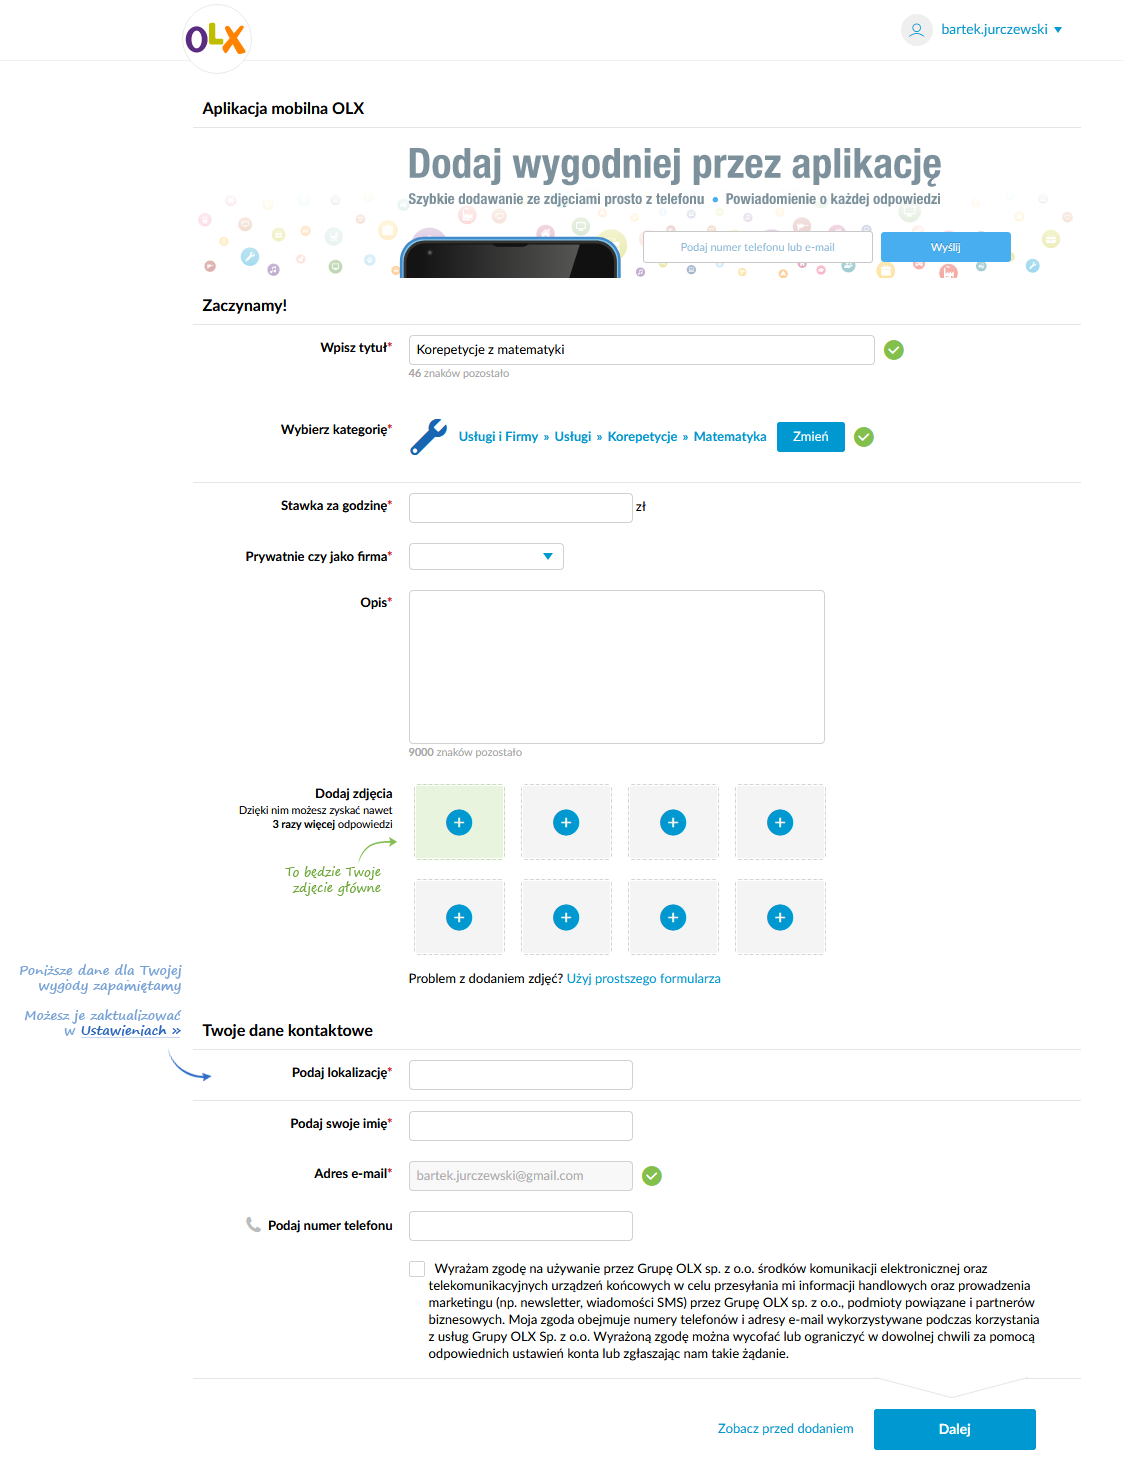
\includegraphics[width=1\textwidth]{{images/olx-dodaj_ogloszenie.png}}
	\caption{Dodawanie ogłoszenia na serwisie OLX}
    \end{figure}

Użytkownik ma do wypełnienia następujące pola:
\begin{itemize}
    \item Tytuł
    \item Kategoria (w tym przypadku Usługi)
    \item Stawka za godzinę
    \item Jakim jest podmiotem gospodarczym
    \item Opis
    \item Dodanie zdjęć
    \item Dane kontaktowe (lokalizacja, imię, nazwisko, adres e-mail, numer telefonu)
\end{itemize}

Jedynym polem które wyróżnia usługę od przedmiotu jest pole "stawka za godzinę". Zgodnie z ideą tego serwisu, użytkownik nie ma możliwości dodania oceny/recenzji po skorzystaniu z jakiejkolwiek usługi, a co za tym idzie porównania ich po ocenach. Dodatkowo serwis ten, całkowicie odrzuca element płatności internetowych (w opozycji do eBaya czy Allegro) i polega wyłącznie na płatności gotówką. Płatności przelewami między użytkownikami są odradzane przez sam OLX, ale są oczywiście możliwe z teoretycznego punktu widzenia. Nie ma jednak wtedy żadnej gwarancji że do takiej wymiany dojdzie, ani możliwości reklamacji czy zwrotu po np. słabo wykonanej usłudze czy otrzymaniu produktu niezgodnego z opisem. Odpowiedzią rynku i rozwoju technologicznego są płatności przez internet.

\subsection{Płatności internetowe i ich bezpieczeństwo} \label{sec:payments}
Rewolucja cyfrowa dotknęła nie tylko rynku usług i produktów ale także rynku płatności. W samym roku 2016 tylko 16\% kupujących w Polsce opłaciło swoje zakupy gotówką \cite{gotowka}. Liczba rozwiązań płatności internetowych rośnie z każdym rokiem. Aktualnie na rynku jest ich kilka. Każde z nich różni się pod względem komfortu użytkowania, szybkości jak i bezpieczeństwa. 
% Najpopularniejsze z nich to:

\subsubsection{Zwykły przelew bankowy}
Jest to najprostsze i najbardziej analogowe rozwiązanie. Zaraz po złożeniu zamówienia, dostajemy potwierdzenie mailem wraz z numerem konta sprzedawcy, kwoty zamówienia i tytułem przelewu (który najczęściej jest numerem zamówienia). Na kupującym ciąży zalogowanie się na stronę banku, utworzenie nowego przelewu i co istotne wypełnienie ich danymi. Oprócz możliwości pomyłki np. przekopiujemy nie pełny numer zamówienia pomijając jeden znak, ryzykiem o którym musimy pamiętać jest obecność złośliwego oprogramowania. Przykładem może być głośna sprawa z roku 2018, w którym to firma ESET natrafiła na konia trojańskiego - BackSwap. Portal \url{www.zaufanatrzeciastrona.pl} opisuje go następująco: "Do wstrzyknięcia dochodzi w momencie, gdy klient zleca przelew. Złośliwy kod podmienia wtedy numer rachunku, na który ma zostać wysłany przelew ofiary. Na ekranie komputera tego nie widać – zmiana dotyczy informacji, które przeglądarka wysyła do banku. Przestępcy nie atakują wszystkich przelewów – definiują konkretny przedział kwotowy, który ich interesuje. Ostatnio celowali w kwoty między 10 000 a 20 000 PLN."\cite{backswap}.
Takie ataki są niestety ciągle spotykane. Niektóre banki jak np. ING Bank Śląski, po skopiowaniu numeru rachunku bankowego usuwa dwie pierwsze cyfry i prosi klienta o uzupełnienie ich. Bank próbuje wymusić podwójne sprawdzenie numeru konta. Efektem ubocznym będzie możliwość pomyłki przy ponownym wprowadzaniu go.

Szybkość takiego rozwiązania jest zależna od godziny wysłania przelewu. Jest to spowodowane godzinami sesji rozliczeniowych w danych bankach. Najczęściej jeśli przelew zostanie wysłany do południa, dotrze on pod wieczór. W przypadku późniejszych przelewów, dojdzie on kolejnego dnia roboczego. Wszystkie przelewy w święta i weekendy również dochodzą dopiero kolejnego dnia roboczego. Taka płatność opóźnia wysyłkę/realizację usługi, ponieważ zostanie ona wykonana dopiero wtedy gdy na rachunku pojawią się przelane środki. 

\subsubsection{Przelewy pay-by-link}
Ta forma płatności cieszy się największą popularnością w Polsce \cite{jak-placa-polacy}. Po wykonaniu zakupów, wybieramy opcję przelewu online, następnie z listy banków, pokazanych na rysunku \ref{fig:pay-by-link} wybieramy ten z którego chcemy dokonać płatności. 

\begin{figure}[H] 
 	\centering
	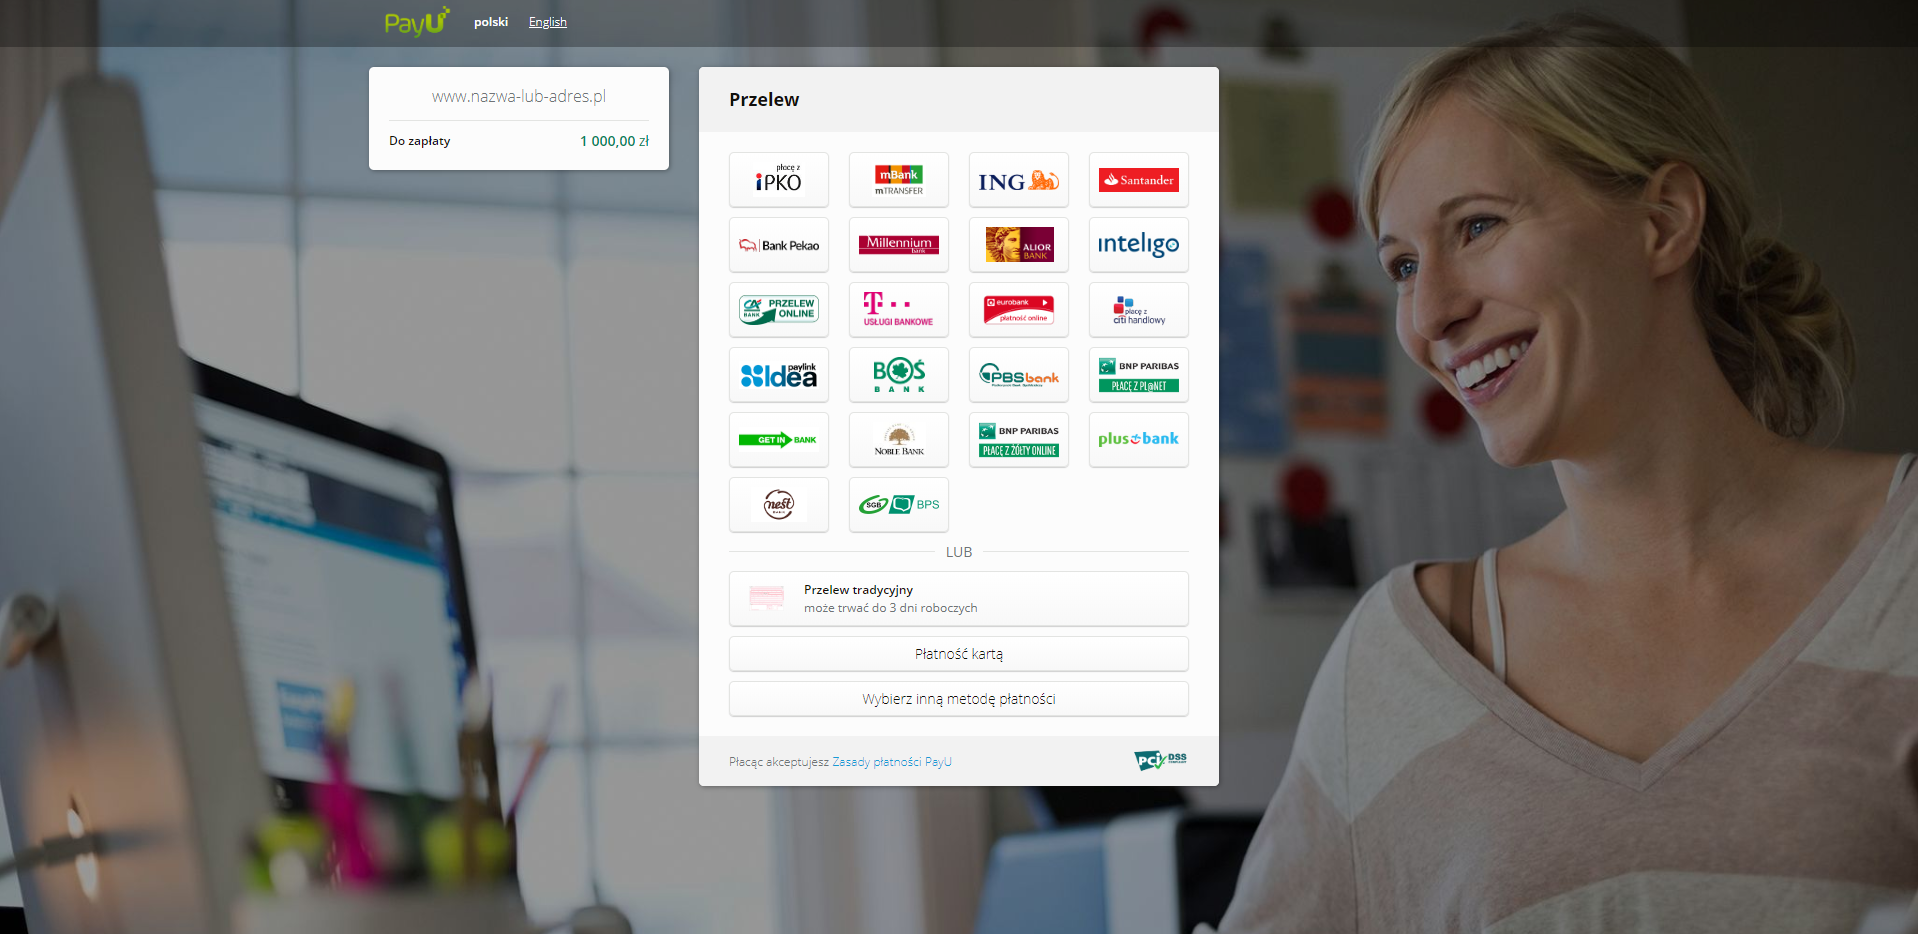
\includegraphics[width=1\textwidth]{{images/przelew-online.png}}
	\caption{Przykładowa płatność pay-by-link}
	\label{fig:pay-by-link}
\end{figure}

Po kliknięciu zostajemy przeniesieni na stronę logowania do danego banku. Po wpisaniu loginu i hasła, pojawi się uzupełniony szablon przelewu który kupujący musi tylko zatwierdzić. Ostatnim krokiem, kluczowym od strony bezpieczeństwa jest SMS z kodem autoryzacyjnym który otrzymamy. Klient musi przepisać owy kod aby potwierdzić przelew. Dzięki temu nawet, jeśli ktoś poznał nasze dane logowania, nie będzie ich mógł użyć do płatności bez posiadania naszego telefonu. Alternatywnym i co raz bardziej popularnym rozwiązaniem jest potwierdzenie przelewu przez aplikację banku. Za nim jednak będzie to możliwe, użytkownik musi się do niej zalogować, co oznacza dodatkowy etap bezpieczeństwa.

Po poprawnym uwierzytelnieniu i potwierdzeniu transakcji, środki trafią niemal natychmiast do sprzedawcy, dzięki czemu od razu będzie wstanie zrealizować zamówienie.

\subsubsection{Karta płatnicza} \label{sec:cards}
W maju 1898 firma Sequoia Data Corp. wprowadziła na rynek Compumarket, pierwszy internetowy system e-commerce obsługujący płatności kartą kredytową. Od tego czasu płatności kartą zyskały wiele nowych usprawnień jednak ich rdzeń pozostał nietknięty. Aby zrealizować płatność, kupujący jest proszony o wpisanie trzech danych: numeru karty, daty jej ważności oraz trzycyfrowego kodu CVC/CVV znajdującego się na odwrocie karty. Po ich zweryfikowaniu, płatność zostaje zakończona. Ta metoda jest tak samo szybka jak pay-by-link ale mniej wygodna, ponieważ za każdym razem musimy ponownie wpisać dane karty. 

Tradycyjny model zakładał nasze zaufanie do portalu w którym dokonujemy zakupów, ponieważ osoba posiadająca owe dany karty mogła samodzielnie dokonać płatności bez naszej zgody. Odpowiedzią na to jest coraz częściej obecna usługa bankowa 3D Secure. Polega ona na dodatkowym etapie weryfikacji. Po poprawnym wpisaniu danych karty i ich zweryfikowaniu, klient otrzymuje SMSa z kodem weryfikacyjnym. Dopiero po wprowadzeniu go, transakcja jest finalizowana.

Zaletą która wyróżnia ten rodzaj płatności jest usługa chargeback. Portal \url{www.najlepszekonto.pl} opisuje ją następująco: "Chargeback, czyli obciążenie zwrotne, to usługa dostępna tylko dla kart płatniczych. Polega ona na zwrocie środków z konta sprzedawcy, jeśli kupiony przez Ciebie towar nie spełnił Twoich oczekiwań: miał wady, różnił się od tego, co obiecywał sprzedawca, lub w ogóle go nie otrzymałeś. Jeśli próby wymiany towaru w sklepie nie powiodą się, możesz zwrócić się z prośbą o rozstrzygnięcie sprawy przez bank, który jest wystawcą Twojej karty."\cite{chargeback}.

Odmianą fizycznej karty płatniczej jest karta wirtualna. Taka karta usłuży tylko do płatności internetowych. Nie użyjemy jej np. podczas zakupów w sklepie. Po jej wyrobieniu, bank nie przesyła nam jej pocztą, a po prostu podaje nam ich dane (numer, data ważności i kod CVC/CVV). Niewątpliwą zaletą jest bezpieczeństwo - nie padniemy ofiarą skimmingu (nielegalne skopiowanie zawartości paska magnetycznego w celu utworzenia kopii). Główną wadą takie rozwiązania jest dostępność w Polsce. Aktualnie tylko dwa banki udostępniają taką usługę - i to za miesięczną opłatą. 

Zagranicznymi serwisami które utworzenie wirtualnych kart, jest np. amerykański \url{www.privacy.com}. Portal ten pozwala na proste i nielimitowane tworzenie kart wirtualnych, jak możemy przeczytać na stronie firmy, "jednym kliknięciem". Klient ma możliwość tworzenia karty per portal (np. jedna karta do Netflixa, kolejna do opłacenia Spotify), dodatkowo może ustawić limit obciążenia dla danej strony, wstrzymać płatność lub całkowicie zablokować niechciane opłaty. 

% \subsubsection{BLIK}
\subsubsection{Portfele elektroniczne}

Hybrydą wymienionych wcześniej rozwiązań są portfele elektroniczne zwane również portfelami cyfrowymi. Rozwiązanie te charakteryzuje się następującymi funkcjonalnościami: 
portfel wirtualny (rozumiany jako pula środków do wykorzystania) wraz z możliwością przelania ich bezpośrednio na rachunek bankowy, płatność wieloma podpiętymi kartami (kredytowymi jak i debetowymi), także w innych walutach, możliwość określenia adresu dostawy klienta i innych informacji ułatwiających sfinalizowanie zamówienia. Kolejnym udogodnieniem jest przechowywanie środków w różnych walutach, dzięki czemu użytkownik nie jest obciążony podwójnym przewalutowaniem.

Niektóre portfele oferują też świadczenie usług bez jakikolwiek przelanych środków i potrafią służyć jako zaufany pośrednik płatności. Jeśli tylko mamy podpiętą kartę/karty pod taki portfel, możemy w dowolnym miejscu zapłacić owym portfelem, a należność zostanie ściągniętą natychmiast z naszej wybranej karty. Dzięki czemu nie jesteśmy wystawieni na potencjalne wady używania samej karty jako środka płatności opisanych w rozdziale \ref{sec:cards}.

\subsection{Obecne rozwiązania}
Przez lata rozwiązania na rynku usług jak i płatności ewoluowały. Często stając się osobnym bytem, a nie dodatkiem jak na początku ich istnienia. Firmy odpowiedzialne za nie, przez lata starały się udoskonalić swój produkt i jak najlepiej go wypromować. Poniższe zestawienie zostało podzielone na dwie grupy: płatności (jako rdzeń serwisu usług) i serwisy dla korepetytorów.

\subsubsection{Płatności}
Szukając odpowiedniego rozwiązania do obsługi płatności, autor miał na celu trzy główne cechy: szybkość (jak szybko środki trafią na konto), wygodę (a w tym szybkość wykonania samej płatności) i bezpieczeństwo (transakcji jak i procesów około transakcyjnych). Każde z czterech dostępnych rozwiązań zostało szczegółowo opisane w rozdziale \ref{sec:payments}, właśnie pod kątem tych trzech cech. Stosując takie kryterium, autor uznaje portfel elektroniczny jako zwycięzce w tych trzech kategoriach. Dlatego w dalszym rozważaniu obecnych rozwiązań będzie brał tylko je pod uwagę.

\begin{table}[H]
\begin{tabular}{|p{5cm}|c|c|c|}
\hline
 & \multicolumn{1}{l|}{\textbf{PayPal}} & \multicolumn{1}{l|}{\textbf{Visa Checkout}} & \multicolumn{1}{l|}{\textbf{Masterpass}} \\ \hline
Język polski & \cmark & \cmark & \cmark \\ \hline
Podpięcie adresu dostawy & \cmark & \cmark & \cmark \\ \hline
Uwierzytelnianie mailem & \cmark & \cmark & \xmark \\ \hline
Używanie kart różnych firm & \cmark & \xmark & \xmark \\ \hline
Możliwość dwustopniowego uwierzytelniania & \cmark & \xmark & \cmark \\ \hline
Możliwość przechowywania środków w portfelu & \cmark & \xmark & \xmark \\ \hline
\end{tabular}
\caption{Porównanie portfeli elektronicznych}
\label{tab:portfele}
\end{table}

Zestawienie pokazane w tabeli \ref{tab:portfele} pokazuje, że PayPal wygrywa w dwóch funkcjonalnościach z Visa Checkout i Masterpassem: użycie kart różnych firm i możliwość przechowywania środków w portfelu.

Ponadto, VisaCheckout i Masterpass są realizowane jako zamknięte środowiska płatnicze. Po kliknięciu na przycisk oznaczony ich logiem, zostajemy przeniesieni do realizacji płatności. PayPal zdecydował się na inne rozwiązanie. Ich rozwiązanie daje klientowi możliwość zapłaty kartą (Visa, MasterCard i Amex), polskim portalem Przelewy24 (który agreguje płatności pay-by-link i kartą - omówione w rozdziale \ref{sec:payments}) i portfelem cyfrowym PayPal. 

\begin{figure}[H] 
 	\centering
	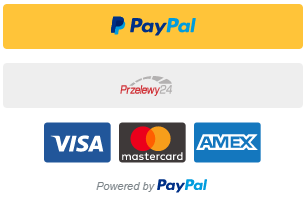
\includegraphics[scale=1.0]{{images/paypal-button.png}}
	\caption{Smart Payment Button}
	\label{fig:paypal-button}
\end{figure}

PayPal określa swój przycisk jako \textbf{Smart Payment Button} (ang. 
inteligentny przycisk do płatności), przedstawiony na rysunku \ref{fig:paypal-button}. Oprócz łączenia kilku sposobów płatności, może różnić się on w każdym kraju. Np. w Polsce wspiera on portal Przelewy24. Dzięki elastyczności \textit{smart payment button} możemy być pewni że zostanie on dostosowany do kraju z którego zostaje dokonywane zamówienie, co potencjalnie może zwiększyć zyski ze względu na bogactwo opcji płatności. 

Podsumowując, w grupie portfeli elektronicznych, rozwiązanie PayPal wspiera wszystkie kluczowe i istotne dla mnie funkcjonalności. Dlatego też, to ono zostanie zaimplementowane w aplikacji \textit{Find-A-Tutor} w celu wspierania płatności on-line.

\subsubsection{Serwisy dla korepetytorów}
Na rynku polskim są obecnie trzy największe serwisy dla korepetytorów. Są to www.e-korepetycje.net, 
korepetycje.net i wspomniany już wcześniej portal, nie tylko do korepetycji - olx.pl. Poniżej zestawiono ze sobą cechy tych portali. Cechy zostały zaczerpnięte z rozdziału \ref{sec:problematyka} pokrywającego problematykę pracy.

\begin{table}[H]
\begin{tabular}{|p{5cm}|c|c|c|c|}
\hline
 & \multicolumn{1}{l|}{e-korepetycje.net} & \multicolumn{1}{l|}{korepetycje.net} & \multicolumn{1}{l|}{olx.pl} \\ \hline
Możliwość płatności online & \xmark & \xmark & \xmark \\ \hline
Ogłoszenia dodawane przez uczniów & \cmark & \xmark & \cmark \\ \hline
Minimalistyczny design & \cmark & \xmark & \xmark \\ \hline
Otwarte API & \xmark & \xmark & \xmark \\ \hline
Aplikacja mobilna & \xmark & \xmark & \cmark \\ \hline
\end{tabular}
\caption{Porównanie serwisów dla korepetytorów}
\label{tab:korepetycje}
\end{table}

Żaden z portali zestawionych powyżej nie obsługuje funkcjonalności tak podstawowej w dzisiejszym świecie jak płatności elektroniczne. Tylko jeden z nich oferuje przyjazny dla oka i wpisujący się w obecne trendy - minimalisty design. Dodatkowo e-korepetycje.net i korepetycje.net nie posiadają otwartego API, które może posłużyć do stworzenia w przyszłości aplikacji mobilnych. Jednym portalem który ją dostarcza, jest OLX.pl.
\newline
\newline
\textit{Obserwując rynek korepetycji, brakuje na nim rozwiązania które wspiera płatności online. Taką aplikacją jest Find-A-Tutor. Dodatkowo, backend został stworzony jako otwarte API, dzięki czemu w przyszłości serwis będzie otwarty na powstanie aplikacji mobilnych. Fundamentalną funkcjonalnością będzie dodawanie ogłoszeń przez studentów. Całość została spięta minimalistycznym i nieprzytłaczającym designem.}

\section{Techniczne aspekty „Find-A-Tutor”}
% http://www.commint.pl/baza/wymagania-niefunkcjonalne-aplikacji-internetowej
% http://www.commint.pl/baza/wymagania-funkcjonalne-aplikacji-internetowej


    \subsection{Wymagania}
    W tym rozdziale autor opisuje wymagania aplikacji webowej \textit{Find-A-Tutor}, dzieląc je na funkcjonalne i niefunkcjonalne. 
        \subsubsection{Wymagania funkcjonalne}
        Jak możemy przeczytać na \url{www.commint.pl}: "Wymagania funkcjonalne aplikacji to określenie jak ma się ona zachować po otrzymaniu określonego zapytania."\cite{funkcjonalne}. Dlatego autor skupił się na określeniu funkcji aplikacji, użytkowników (wraz z ich rolami i uprawnieniami), problemów jakie aplikacja ma rozwiązywać jak i ogólnej wizji aplikacji.\\
        \noindent
        \textbf{Rejestracja jako uczeń lub korepetytor}\\
        \indent
        Formularz rejestracji pozwala na rejestrację jako użytkownik z wyróżnieniem ucznia i użytkownika. Oba ta konta moją inne uprawnienia i funkcjonalności opisane poniżej.
            
        \noindent
        \textbf{Logowanie jako uczeń, korepetytor i administrator}\\
        \indent  
        Dostępny panel logowania dla użytkownika (ucznia lub korepetytora). Dodatkowym rodzajem konta jest administrator, który ma pełne uprawnienia do działania na systemie. Takie konto nie posiada panelu użytkownika, ale może dokonywać wszelakich operacji opisanych w osobnym punkcie, używając zapytań do API.
            
        \noindent
        \textbf{Panel ucznia}\\
        \indent
        Panel dostępny dla użytkownika zalogowanego jako student. Umożliwia podgląd wszystkich ogłoszeń zgłoszonych przez danego ucznia. Dodatkowo powinien on wyświetlać podstawowe dane takie jak: data utworzenia, datę podjęcia ogłoszenia, opis, datę wygaśnięcia ogłoszenia, przedmiot, status płatności i status ogłoszenia. Logowanie następuje przez przeglądarkę internetową. 
        
        \noindent
        \textbf{Podgląd szczegółów ogłoszenia}\\
        \indent
        Uczeń powinien mieć dostęp do widoku szczegółowego ogłoszenia, który pokazuje wszystkie informacje na temat ogłoszenia.
        
        \noindent
        \textbf{Dodawanie ogłoszeń}\\
        \indent
        Możliwość dodania ogłoszenia przez użytkownika - ucznia. Użytkownik uzupełnia następujące dane: opis, data przedawnienia ogłoszenia, przedmiot (wybrany z listy przedmiotów). 
        
        \noindent
        \textbf{Płatności online za lekcje}\\
        \indent
        Po przypisaniu ogłoszenia do korepetytora, student ma możliwość opłacenia należności za ogłoszenie online. Po opłaceniu, ma to odzwierciedlenie w statusie. 
        
        \noindent
        \textbf{Finalizacja ogłoszenia}\\
        \indent
        Po odbytej lekcji, użytkownik zaznacza zakończenie takiej lekcji, tym samej zmieniając jej status.
        
        \noindent
        \textbf{Panel korepetytora}\\
        \indent
        Użytkownik korepetytor, po zalogowaniu ma dostęp do swojego panelu ze wszystkimi dostępnymi ogłoszeniami i ze wszystkimi podjętymi przez niego ogłoszeniami. Dostępne są na nim następujące informacje: data utworzenia, datę podjęcia ogłoszenia, opis, datę wygaśnięcia ogłoszenia, przedmiot, status płatności i status ogłoszenia. Logowanie następuje przez przeglądarkę internetową. 
        
        \noindent
        \textbf{Podjęcie ogłoszenia}\\
        \indent
        Korepetytor ma możliwość podjęcie ogłoszenia z puli nieprzydzielonych ogłoszeń. Podaje on swoją stawkę godzinową wyrażoną w złotówkach. Stawka ta zostaje przypisana do ogłoszenia wraz z kwotą należną za całe ogłoszenie (stawka pomnożona przez liczbę godzin). Po operacji podjęcia, zmienia on swój status.
        
        \noindent
        \textbf{Oddanie ogłoszenia}\\
        \indent
        Jeśli ogłoszenie, po podjęciu, nie zostało jeszcze opłacone, korepetytor ma możliwość zwrócenia ogłoszenia do ogólnej puli ogłoszeń., tym samym jego status wraca do stanu wejściowego. 
        
        \noindent
        \textbf{Konto administratora}\\
        \indent
        Po zalogowaniu się zapytanie, taki użytkownik może wykonywać operacje CRUD (ang. create, read, update and delete (pol. utwórz, odczytaj, aktualizuj i usuń)) na ogłoszeniach, użytkownikach i przedmiotach. Dodatkowo ma możliwość wszystkich operacji ucznia czy korepetytora.
        
        \subsubsection{Wymagania niefunkcjonalne}
        
        Jak możemy przeczytać na \url{www.commint.pl}: "Wymagania niefunkcjonalne aplikacji internetowej dotyczą obszaru jakościowego tworzonego rozwiązania."\cite{niefunkcjonalne}. Dlatego autor skupił się na przenośności, skalowalności, otwartości na rozszerzenia, kompatybilności, bezpieczeństwu, użyteczności i modularności.\\
        \noindent
        \textbf{Przenośność}\\
        \indent
        Aplikacja powinna być łatwa w zmianie lokalizacji, środowiska, eksportu danych.
        
        \noindent
        \textbf{Skalowalność}\\
        \indent
        Aplikacja powinna móc się skalowalność pionowo (zwiększenie mocy serwera) i poziomo (zwiększenie instancji aplikacji).
        
        \noindent
        \textbf{Otwartość na rozszerzenia}\\
        \indent
        Aplikacja powinna mieć otwarte API (backend) i być gotowa na nowe urządzenia które mogą z niej korzystać (np. mobilne).
        
        \noindent
        \textbf{Kompatybilność}\\
        \indent
        Aplikacja powinna działać w technologiach uniwersalnych i powszechnych dla przeglądarkę na silniku Chromium (Chrome, Opera i wkrótce Edge), który na rynku polskim ma 80,65\% podziału rynku \cite{chrome}.
        
        \noindent
        \textbf{Bezpieczeństwo}\\
        \indent
        Dane użytkowników powinny być poufne i dostępne dla danego użytkownika po zalogowaniu.
        
        \noindent
        \textbf{Użyteczność }\\
        \indent
        Aplikacja powinna być łatwa w obsłudze i powinna być okraszona minimalistycznym designem który nie przytłacza użytkownika.
        
        \noindent
        \textbf{Modularność}\\
        Warstwa bazy danych, graficzna i aplikacji (API) powinny być od siebie oddzielone i gotowe do zastąpienia.
        
    \subsection{Architektura aplikacji}
    % https://www.c-sharpcorner.com/article/onion-architecture-in-asp-net-core-mvc/
    % https://www.youtube.com/watch?v=_lwCVE_XgqI
        \subsubsection{API}
        \subsubsection{Rdzeń}
        \subsubsection{Infrastruktura}
    \subsection{Warstwa bazy danych}
    \subsection{Warstwa graficzna}
\section{Aplikacja z poziomu użytkownika}
\section{Wnioski}

    \clearpage
    
     % lista obrazków - generuje się automatycznie
    \section{Indeks rysunków}
        \listoffigures
    \clearpage    
    
    % lista tabel - generuje się automatycznie
    \section{Indeks tabel}
        \listoftables
    \clearpage
    
    \section{Bibliografia}
    \renewcommand{\section}[2]{}
    \begin{thebibliography}{9}
    % linki bibliograficzne do źródeł internetowych typu link, itp
    \bibitem{internet-users} 
    World Internet Users and 2019 Population Stats
    \url{https://www.internetworldstats.com/stats.htm}, dostęp 24-11-2019

    \bibitem{computers} 
    Computers sold this year
    \url{https://www.worldometers.info/computers/}, dostęp 24-11-2019
    
    \bibitem{ranking} 
    Ranking sklepów internetowych 2019
    \url{http://static.opineo.pl/press/dl/ranking-sklepow-internetowych-opineo-2019.pdf}, dostęp 28-11-2019
    
    \bibitem{allegro-wywiad} 
    Bakker o Allegro.pl: Cel był jasny. W e-commerce mógł być tylko jeden gracz
    \url{https://polskatimes.pl/bakker-o-allegropl-cel-byl-jasny-w-ecommerce-mogl-byc-tylko-jeden-gracz/ar/664791}, dostęp 28-11-2019
    
    \bibitem{allegro-liczby} 
    Wyniki badania Gemius/PBI za lipiec 2017
    \url{https://www.gemius.pl/wydawcy-aktualnosci/wyniki-badania-gemiuspbi-za-lipiec-2017.html}, dostęp 28-11-2019
    
    \bibitem{olx-wywiad} 
    Meet OLX, the biggest Web company you’ve never heard of
    \url{https://fortune.com/2014/10/29/olx-emerging-markets/}, dostęp 28-11-2019
    
    \bibitem{olx-liczby} 
    Wyniki badania Gemius/PBI za styczeń 2019
    \url{https://www.gemius.pl/wszystkie-artykuly-aktualnosci/wyniki-badania-gemiuspbi-za-styczen-2019.html}, dostęp 28-11-2019
    
    \bibitem{gotowka} 
    Sondaż: Jak Polacy płacą w Internecie?
    \url{https://www.kir.pl/o-nas/aktualnosci/sondaz-jak-polacy-placa-w-internecie,142.html}, dostęp 30-11-2019
    
    \bibitem{backswap} 
    Klienci PKO BP, BZ WBK, mBanku, ING i Pekao na celowniku nowego malware
    \url{https://zaufanatrzeciastrona.pl/post/klienci-pko-bp-bz-wbk-mbanku-ing-i-pekao-na-celowniku-nowego-malware/}, dostęp 30-11-2019
    
    \bibitem{jak-placa-polacy} 
    Jak Polacy kupują i płacą przez internet? Co lubią, czego się boją?
    \url{https://www.shoper.pl/blog/jak-polacy-kupuja-i-placa-przez-internet/}, dostęp 1-12-2019
    
    \bibitem{chargeback} 
    Płatność kartą przez Internet
    \url{https://www.najlepszekonto.pl/platnosc-karta-przez-internet}, dostęp 2-12-2019
    
    \bibitem{funkcjonalne} 
    Wymagania funkcjonalne aplikacji internetowej
    \url{http://www.commint.pl/baza/wymagania-funkcjonalne-aplikacji-internetowej}, dostęp 10-12-2019
        
    \bibitem{niefunkcjonalne} 
    Wymagania niefunkcjonalne aplikacji internetowej
    \url{http://www.commint.pl/baza/wymagania-niefunkcjonalne-aplikacji-internetowej}, dostęp 10-12-2019
    
    \bibitem{chrome} 
    Browser Market Share Poland
    \url{https://gs.statcounter.com/browser-market-share/all/poland}, dostęp 10-12-2019
    
    % linki bibliograficzne do ksiazek
    % \bibitem{book1} 
    % Amir Vahid Dastjerdi, Rajkumar Buyya.
    % \textit
    % Internet of Things. Morgan Kaufmann, 2016.
    \end{thebibliography}

\end{document}